% --------------------- VARIABLEN -------------------------

\newcommand{\COURSE}{Physik und Materialwissenschaften\\ Praktikum Physik \\}
\newcommand{\SEMESTER}{Elektro- und Informationstechnik II}
\newcommand{\STUDENT}{Maximilian Spahn\\ und\\Benjamin Langer}

\newcommand{\HEADDING}{Praktikum Physik}
\newcommand{\SUBHEADDING}{Versuch 2.1: Schwingungen}

% ------------------- DEFINITIONEN -----------------------

\documentclass[a4paper]{scrartcl}

\usepackage[utf8]{inputenc}
\usepackage[ngerman]{babel}
\usepackage{amsmath}
\usepackage{amssymb}
\usepackage{color}
\usepackage{tikz}
\usepackage{float}
\usetikzlibrary{arrows,decorations.markings}
\usepackage{tabularx}
\usepackage{fancybox}
\usepackage{pgfplots}
\usepackage{geometry}
\usepackage{fancyhdr}
\usepackage[page]{totalcount}

%Größe der Ränder setzen
\geometry{a4paper,left=2cm, right=2cm, top=3cm, bottom=2cm, headheight=8cm}

%Kopf- und Fußzeile
\pagestyle {fancy}
\fancyhf{}
\fancyhead[L]{\STUDENT}
\fancyhead[C]{\COURSE}
\fancyhead[R]{\today}

\fancyfoot[L]{\SEMESTER}
\fancyfoot[C]{}
\fancyfoot[R]{Seite \thepage /\totalpages}

%Formatierung der Überschrift, hier nichts ändern
\def\header#1#2{
  \begin{center}
    {\Large #1}\\
    {#2}
  \end{center}
}

\numberwithin{equation}{subsection}

% ----------------------- DOCUMENT ---------------------------

\begin{document}

\vspace{10pt}
\header{\HEADDING}{\SUBHEADDING}

\tableofcontents

\newpage

\section{Häusliche Vorarbeit}
\subsection{Mechanischer Oszillator}
\subsubsection{Aufgabe 3.1.1: Gleichung Rotationsschwinger}

\begin{align}
(m*\dfrac{d^2}{dt} + b*\dfrac{dx}{dt} + k*x = 0)
\end{align}

\begin{align*}
\text{Auslenkung:}& \quad x 							&&\longrightarrow \varphi \\
\text{Masse:}& \quad m   							&&\longrightarrow J \textit{(Trägheitsmoment)} &\\
\text{Geschwindigkeit:}& \quad v=\dfrac{dx}{dt} 		&&\longrightarrow \omega \textit{(Winkelgeschwindigeit)}&\\
\text{Beschleunigung:}& \quad a=\dfrac{d^2x}{dt^2} 	&&\longrightarrow \alpha \textit{(Winkelbeschleunigung)}&
\end{align*}

\begin{align*}
\text{Newton:}& \quad m \cdot a  		&&\longrightarrow J \cdot \alpha = J \dfrac{d\varphi}{dt} &\\
\text{Dämpfungsgrad:}& \quad b \cdot v  	&&\longrightarrow b \cdot \omega = b \dfrac{d^2\varphi}{dt^2} &\\
\text{Beschleunigung:}& \quad k \cdot x 	&&\longrightarrow k \cdot \varphi &
\end{align*}

\begin{align}
\Rightarrow \text{DGL.Torsionsschwinger:} \quad J*\dfrac{d^\varphi}{dt} + b*\dfrac{d\varphi}{dt} + k*\varphi = 0
\end{align}

\subsubsection{Aufgabe 3.1.2: Drehfederkonstante des Schwingers}

Definition Drehfederkonstante:
\begin{align}
M = k \cdot \varphi
\end{align}

Definition Drehmoment:
\begin{align}
M = r \cdot F
\end{align}

Aus Umstellen und Einsetzen der beiden Definitionen erhält man die Federkonstante aus Auslenkung und Kraft am Radius $r$:
\begin{align}
k = \dfrac{r \cdot F}{\varphi}
\end{align}

\begin{table}[H]
\begin{tabular}{|l|l|l|}
\hline
\textbf{$\varphi/rad$} & \textbf{$F/N$} & \textbf{$k/\dfrac{Nmm}{rad}$} \\ \hline
0,6                    & 0,1            & 15,83                         \\ \hline
0,8                    & 1,15           & 17,81                         \\ \hline
1,1                    & 0,2            & 17,27                         \\ \hline
1,3                    & 0,25           & 18,26                         \\ \hline
1,6                    & 0,3            & 17,81                         \\ \hline
1,8                    & 0,35           & 18,47                         \\ \hline
2,0                    & 0,4            & 19                            \\ \hline
2,3                    & 0,46           & 19                            \\ \hline
2,4                    & 0,48           & 19                            \\ \hline
\end{tabular}
\centering
\end{table}

Damit ergibt sich als Mittelwert die Federkonstante:

\begin{align*}
\Rightarrow \text{Federkonstante:} \quad \overline{k} \approx 18,1 \dfrac{Nmm}{rad} = 18,1 \cdot 10^{-3} \dfrac{Nm}{rad}
\end{align*}

\subsubsection{Aufgabe 3.1.3: Bestimmung der Massenträgheitsmomente}

\begin{align}
A_{ges} &= \Pi \cdot r^2 = 28352,87mm^2 \\
A_r &= A_{ges} - A_s = 24872,87mm^2 \\
m_r &= \dfrac{m_{ges}}{A_{ges} \cdot A_r = 22,47g}
\end{align}

Massenträgheitsmoment Hohlzylinder:
\begin{align}
J_r = \dfrac{1}{2} \cdot (r_{\textit{innen}}^2 + r_{\textit{außen}}^2) = 1629,59 kg \cdot mm^2
\end{align}

Massenträgheitsmoment Gesamt:
\begin{align}
J_{ges} = J_{s} + J_{r} = 1829,6 1629,59 kg \cdot mm^2 = 1829,6 \cdot 10^{-6} kg \cdot m^2
\end{align}
	
\subsubsection{Aufgabe 3.1.4: Berechnung der Eigenfrequenz}

Eigenfrequenz:
\begin{align}
\omega_{0,\textit{theor.}} = \sqrt{\dfrac{k}{J}} = 3,145 \dfrac{rad}{s}
\end{align}

Periodendauer:
\begin{align}
T_{0,\textit{theor.}} = \dfrac{2\Pi}{\omega_{0,\textit{theor.}}} = 1,99s
\end{align}

\subsection{Elektrischer Oszillator}
\subsubsection{Aufgabe 3.2.1: Ersatzwiderstand der Spule}

Eine Spule besteht aus einem (dünnen) gewickelten Draht, welcher selbst einen Leitungswiederstand aufweist.
Dieser kann ersatzweise als Widerstand in Reihe zu der Spule dargestellt werden.

\subsubsection{Aufgabe 3.2.2: Gesamtwiderstand}

bei dem Gesamtwiederstand handelt es sich um eine Reihenschaltung aus dem Innenwiderstand der Spule und den beiden externen Widerständen. 
\begin{align}
R_{ges} = R_1 + R_2 + R_3
\end{align}

Als Ungenauigkeit der externen Widerstände wird $\mp 0,05 k \Omega$ angenommen.

\begin{align*}
R_{3,min} = (0+0,05)k\Omega &\Rightarrow R_{ges,min} = (6,45+0,1)k\Omega \\
R_{3,max} = (10\mp0,05)k\Omega &\Rightarrow R_{ges,min} = (16,45\mp0,1)k\Omega
\end{align*}

\subsubsection{Aufgabe 3.2.3: Eigenfrequenz ohne Dämpfung}

\begin{align}
\omega_{0,\textit{theor.}} = \sqrt{\dfrac{1}{LC}}= 1497,8318 \frac{rad}{s}
\end{align}

Fehlerrechnung:
\begin{align*}
\vert \frac{\partial}{\partial L}\omega_{0,\textit{theor.}}\vert = \frac{LC}{2L^2C} &\\
\vert \frac{\partial}{\partial C}\omega_{0,\textit{theor.}}\vert = \frac{LC}{2LC^2} &
\end{align*}
\begin{align*}
U_{\omega_{0,\textit{theor.}}} = \vert \frac{\partial}{\partial L}\omega_{0,\textit{theor.}}\vert \cdot U_L + \vert \frac{\partial}{\partial C}\omega_{0,\textit{theor.}}\vert \cdot U_C = 140,841 \frac{rad}{s} \approx 150 \frac{rad}{s}
\end{align*}

\begin{align*}
\Rightarrow \omega_{0,\textit{theor.}} = (1490 \mp 150) \frac{rad}{s}
\end{align*}

\subsubsection{Aufgabe 3.2.4: Abklingkoeffizient}

\begin{align}
\delta_{\textit{theor.}} = \dfrac{R}{2L}= 151,3453
\end{align}

Fehlerrechnung:
\begin{align*}
\vert \frac{\partial}{\partial R}\delta_{\textit{theor.}}\vert = \frac{1}{2L} &\\
\vert \frac{\partial}{\partial L}\delta_{\textit{theor.}}\vert = \frac{R}{2L^2} &
\end{align*}
\begin{align*}
U_{\delta_{\textit{theor.}}} = \vert \frac{\partial}{\partial R}\delta_{\textit{theor.}}\vert \cdot U_R + \vert \frac{\partial}{\partial L}\delta_{\textit{theor.}}\vert \cdot U_L = 11,4863 \approx 12 
\end{align*}

\begin{align*}
\Rightarrow \delta_{\textit{theor.}} = (151 \mp 12) \frac{rad}{s}
\end{align*}

\subsubsection{Aufgabe 3.2.5: gedämpfte Eigenfrequenz}

\begin{align}
\omega_{D,\textit{theor.}} = \sqrt{\omega_{0,\textit{theor.}}^2 - \delta_{\textit{theor.}}^2} = 1482,329 \frac{rad}{s}
\end{align}

Fehlerrechnung:
\begin{align*}
\vert \frac{\partial}{\partial \omega_{0,\textit{theor.}}}\omega_{D,\textit{theor.}}\vert = \frac{\omega_{0,\textit{theor.}}}{\sqrt{\omega_{0,\textit{theor.}}^2 - \delta_{\textit{theor.}}^2}} &\\
\vert \frac{\partial}{\partial \delta_{\textit{theor.}}}\omega_{D,\textit{theor.}}\vert = \frac{\delta_{\textit{theor.}}}{\sqrt{\omega_{0,\textit{theor.}}^2 - \delta_{\textit{theor.}}^2}} &
\end{align*}
\begin{align*}
U_{\omega_{D,\textit{theor.}}} = \vert \frac{\partial}{\partial \omega_{0,\textit{theor.}}}\omega_{D,\textit{theor.}}\vert \cdot U_{\omega_{0,\textit{theor.}}} + \vert \frac{\partial}{\partial \delta_{\textit{theor.}}}\omega_{D,\textit{theor.}}\vert \cdot U_{\delta_{\textit{theor.}}} = 151,9716 \approx 160
\end{align*}

\begin{align*}
\Rightarrow \omega_{D,\textit{theor.}} = (1480 \mp 160) \frac{rad}{s}
\end{align*}

\subsubsection{Aufgabe 3.2.6: Gesamtwiderstand beim aperiodischer Grenzfall}

Bedingung für den aperiodischer Grenzfall:
\begin{align}
\text{Aperiodicher Genzfall:} \quad \omega_{0,\textit{theor.}}^2 = \delta_{\textit{theor.}}^2
\end{align}

\begin{align*}
(\omega_{0,\textit{theor.}} \text{ist unabhängig von R}) \quad \text{und} \quad
\delta_{\textit{theor.}} = \frac{R}{2L}
\end{align*}

damit ergibt sich als Gleichung zur Bestimmung des Widerstandes:

\begin{align}
\omega_{0,\textit{theor.}}^2 = \frac{R^2}{4L^2} \quad \Rightarrow \quad R_{\textit{grenz,theor.}} &= \omega_{0,\textit{theor.}} \cdot 2L = 13290,8 \Omega
\end{align}


Fehlerrechnung:
\begin{align*}
\vert \frac{\partial}{\partial \omega_{0,\textit{theor.}}}R_{\textit{grenz,theor.}}\vert = 2 \cdot L &\\
\vert \frac{\partial}{\partial L}R_{\textit{grenz,theor.}}\vert = 2 \cdot \omega_{0,\textit{theor.}} &
\end{align*}
\begin{align*}
U_{R_{\textit{grenz,theor.}}} = \vert \frac{\partial}{\partial \omega_{0,\textit{theor.}}}R_{\textit{grenz,theor.}}\vert \cdot U_{\omega_{0,\textit{theor.}}} + \vert \frac{\partial}{\partial L}R_{\textit{grenz,theor.}}\vert \cdot U_L = 1840,60 \approx 1900 
\end{align*}

\begin{align*}
\Rightarrow R_{\textit{grenz,theor.}} = (13,3 \mp 1,9) k \Omega
\end{align*}

\subsubsection{Aufgabe 3.2.6: Funktion des Tasters}
Der Taster verbindet in seiner Ausgangspostion die Spannungsquelle mit dem Kondensator, sodass dieser geladen wird und so der Schwingung ihre Startenergie zugeführt wird. Wird der Taster betätigt wird die Spannungsversorgung getrennt und der Schwingkreis aus Widerstand, Spule und Kondensator geschlossen, wodurch eine freie gedämpfte Schwingung zwischen Spule und Kondensator stattfindet. Dabei oszilliert die zuvor dem Kondensator zugeführte Energie zwischen den beiden Bauteilen.

\section{Auswertung Versuch}
\subsection{Mechanischer Oszillator}
\subsubsection{Bremsstrom 0A - freie Schwingung}

\begin{figure}[H]
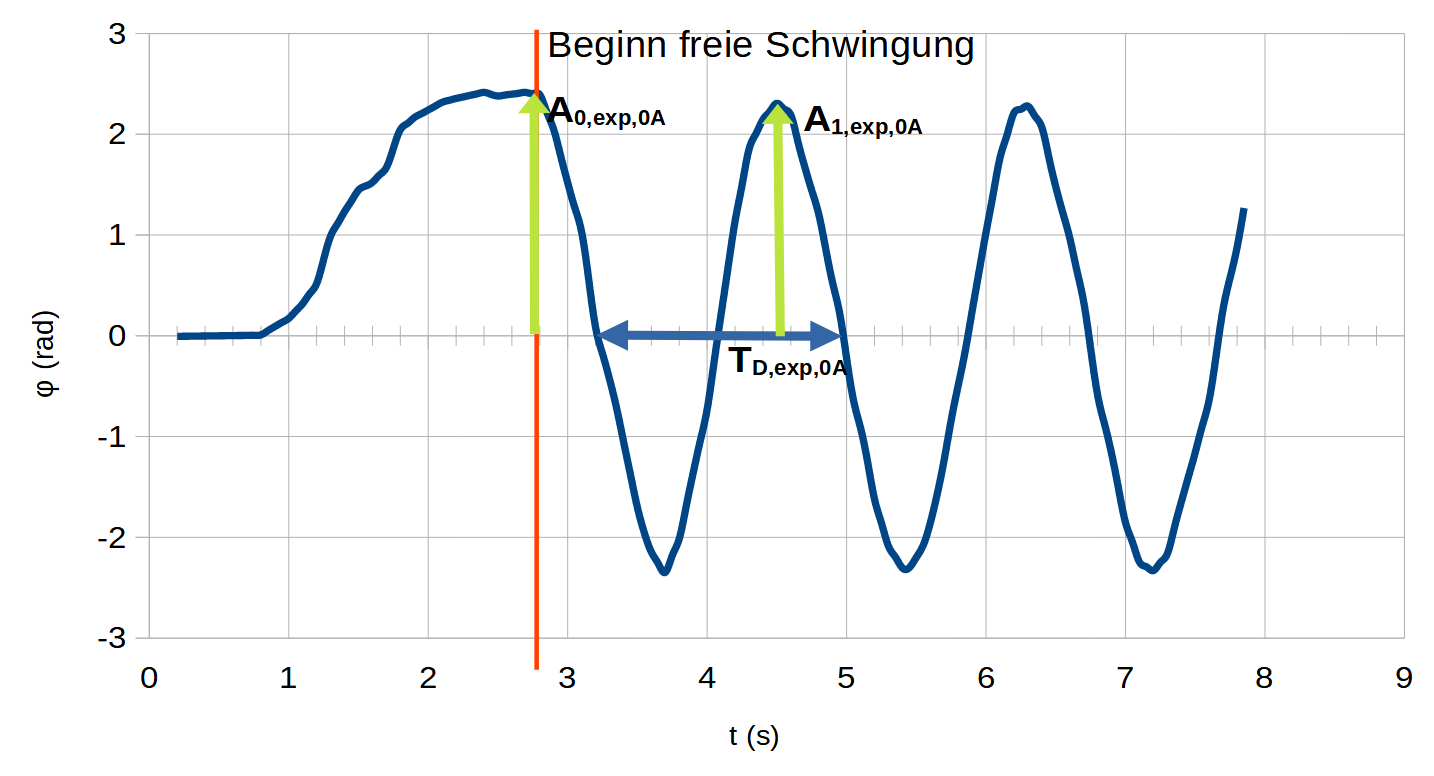
\includegraphics[width=8cm]{Messung_Rad_graph_0A}
\centering
\end{figure}

Bei dem Versuchsdurchlauf handelt es sich um eine freie Schwingung. Die Schwingung verläuft periodisch und die Amplitude nimmt nur wenig (durch den Luftwiederstand und Reibung in den Lagern ist keine vollständig gedämpfte Schwingung möglich) ab, wodurch die Schwingung ungedämpft ist.
\\ \\
\textbf{Aus dem Diagramm lässt sich ablesen:}
\begin{align*}
\text{Periodendauer:} T_{0,\textit{exp.},0A} = (1,80\mp0,10)s \\
\end{align*}
Der Abklingkoeffizient kann nicht genau aus den Messdaten abgelesen werden, da die Dämpfung zu klein und somit $A_{0,\textit{exp.},0A} \approx A_{1,\textit{exp.},0A}$ ist
\\ \\
\textbf{Berechnung der Kreisfrequenz:}
\begin{align}
\omega_{0,\textit{exp.},0A} = \frac{2\pi}{T_{0,\textit{exp.},0A}} = 3,496 \frac{1}{s}
\end{align}

\subsubsection{Bremsstrom 0,5A - gedämpfte Schwingung}

\begin{figure}[H]
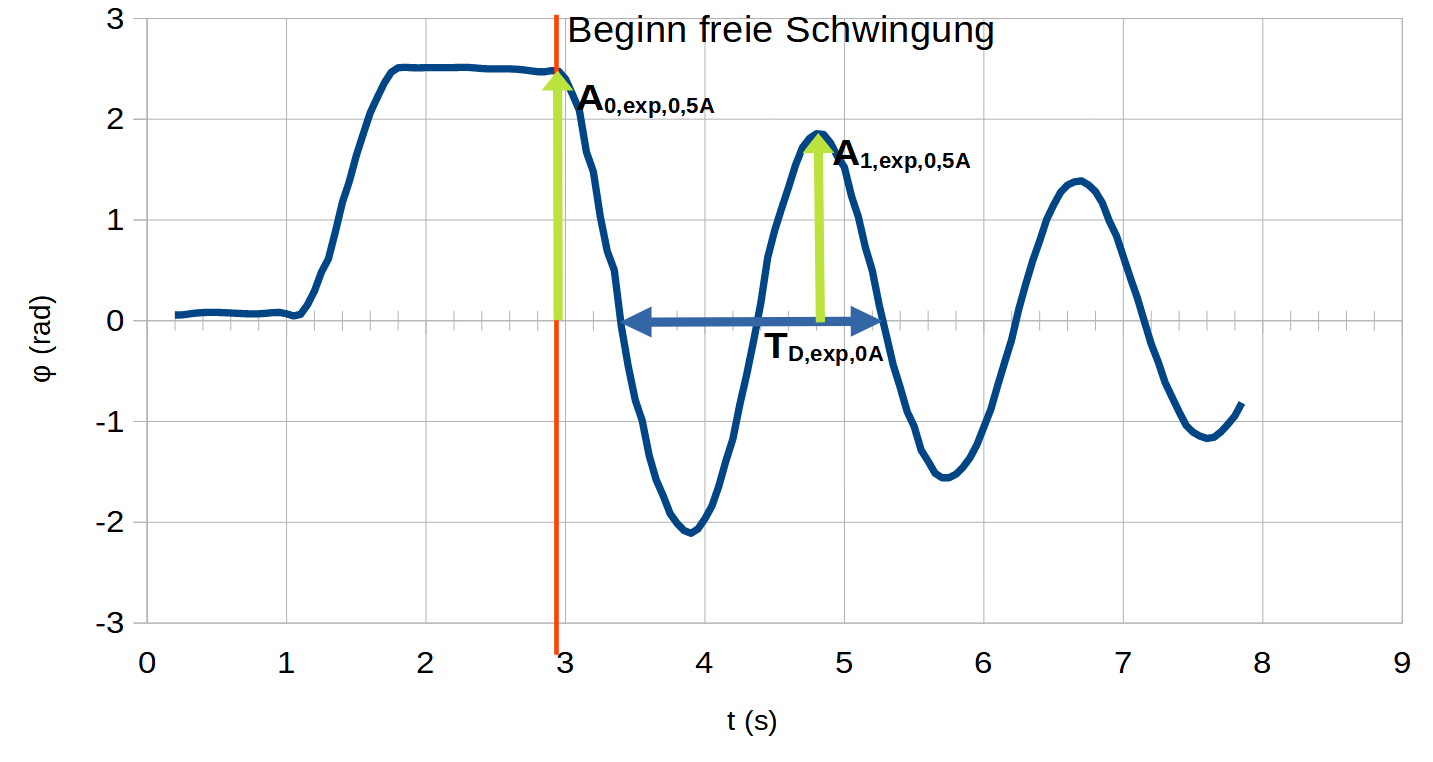
\includegraphics[width=8cm]{Messung_Rad_graph_05A}
\centering
\end{figure}

Bei dem Versuchsdurchlauf handelt es sich um eine gedämpfte Schwingung. Die Schwingung verläuft periodisch und die Amplitude nimmt fortlaufend exponentiell ab, wodurch die Schwingung gedämpft ist. Bei dem Versuch war der Strom der Wirbelstrombremse auf $(0,500\mp0,02)A$ eingestellt, was die Beobachtete Dämpfung hervorrief.
\\ \\
\textbf{Aus dem Diagramm lässt sich ablesen:}
\begin{align*}
\text{Periodendauer:} T_{D,\textit{exp.},0A} = (1,90\mp0,10)s \\
\text{Auslenkung 0. Maxima:} A_{0,\textit{exp.},0,5A} = (2,5\mp0,1)rad \\
\text{Auslenkung 1. Maxima:} A_{1,\textit{exp.},0,5A} = (1,9\mp0,1)rad
\end{align*}

\textbf{Berechnung der gedämpften Kreisfrequenz:}
\begin{align}
\omega_{D,\textit{exp.},0,5A} = \frac{2\pi}{T_{D,\textit{exp.},0,5A}}
\end{align}

\textbf{Berechnung des Logarithmischen Dekrements:}

\begin{align}
\Lambda_{\textit{exp.},0,5A} = \ln(\frac{A_{0,\textit{exp.},0,5A}}{A_{1,\textit{exp.},0,5A}})
\end{align}

\textbf{Berechnung des Abklingkoeffizienten:}

\begin{align}
\delta_{\textit{exp.},0,5A} = \frac{\Lambda_{\textit{exp.},0,5A}}{T_{D,\textit{exp.},0,5A}}
\end{align}

\textbf{Berechnung der Kreisfrequenz des ungedämpften Systems:}

\begin{align}
\omega_{0,\textit{exp.},0,5A} = \sqrt{\omega_{D,\textit{exp.},0,5A}^2 + \delta_{\textit{exp.},0,5A}^2}
\end{align}

\subsubsection{Bremsstrom 2,1A - aperiodischer Grenzfall}

\begin{figure}[H]
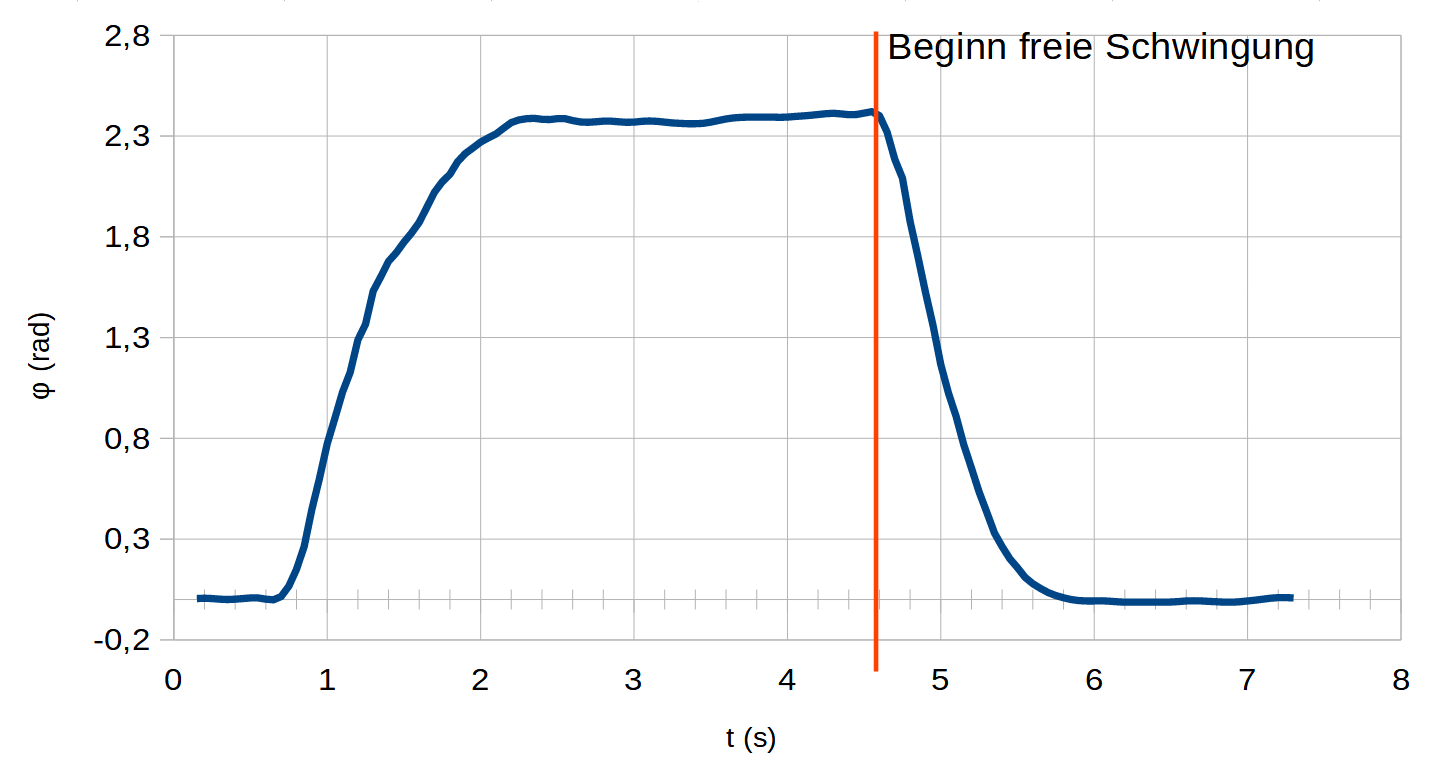
\includegraphics[width=8cm]{Messung_Rad_graph_21A}
\centering
\end{figure}

Bei dem Versuchsdurchlauf handelt es sich um den aperiodischen Grenzfall. Die Schwingung ist so stark gedämpft, dass diese bereits nach einer halben Schwingung zum Stillstand kommt. Dabei beginnt die Schwingung wie die ungedämpfte Schwingung nähert sich dann jedoch der null Position an ohne in negative Richtung über zu schwingen. Bei dem Versuch war der Strom der Wirbelstrombremse auf $(2,100\mp0,020)A$ eingestellt, was die Beobachtete starke Dämpfung hervorrief.

\subsubsection{Bremsstrom 2,5A - Kriechfall}

\begin{figure}[H]
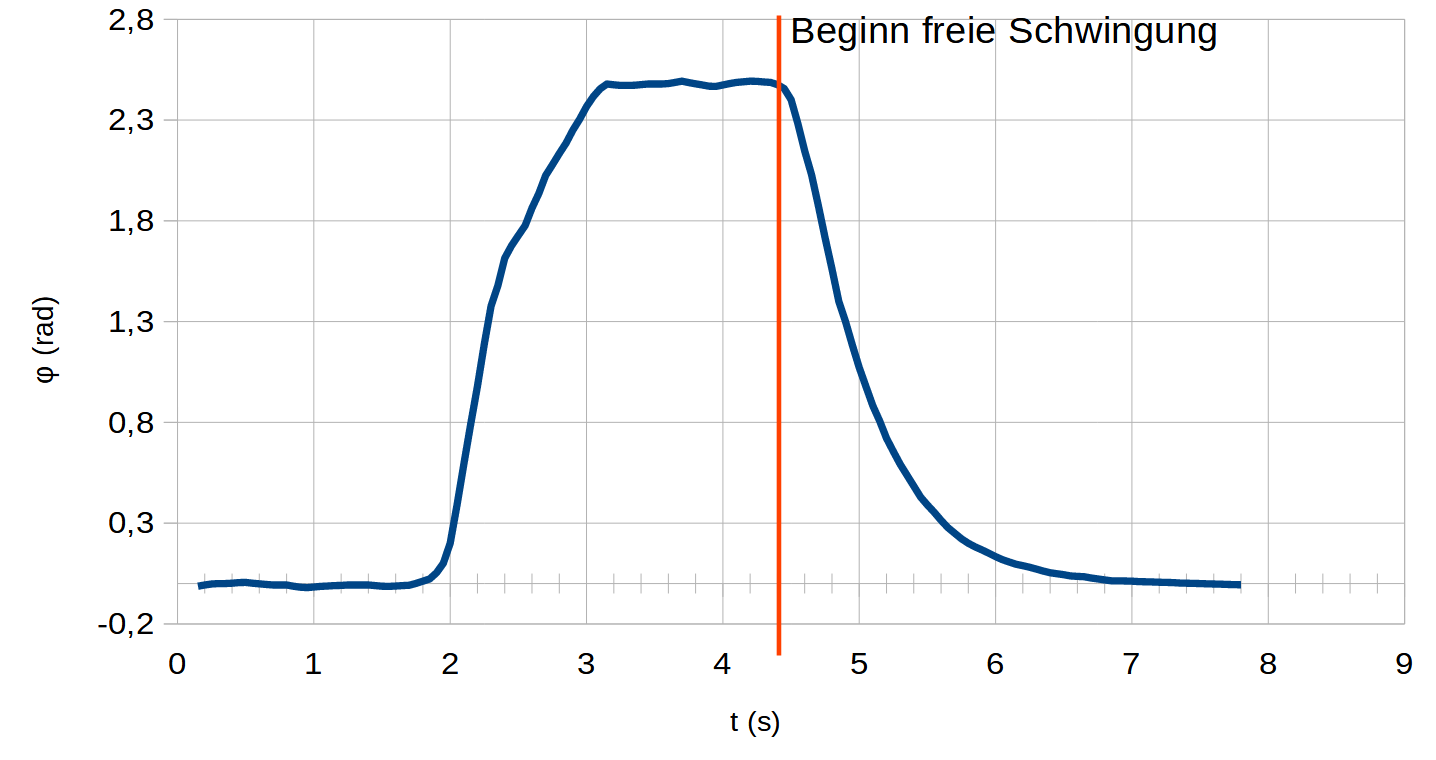
\includegraphics[width=8cm]{Messung_Rad_graph_25A}
\centering
\end{figure}

Bei dem Versuchsdurchlauf handelt es sich um den aperiodischen Grenzfall. Die Schwingung ist so stark gedämpft, kein Schwingendes Verhalten zu erkennen ist. Dabei nähert sich das Rad seiner null Position nur langsam asymptotisch an. Bei dem Versuch war der Strom der Wirbelstrombremse auf $(2,500\mp0,020)A$ eingestellt, was die Beobachtete sehr starke Dämpfung hervorrief.

\subsection{Elektrischer Oszillator}
\subsubsection{Schwingfall}

\begin{figure}[H]
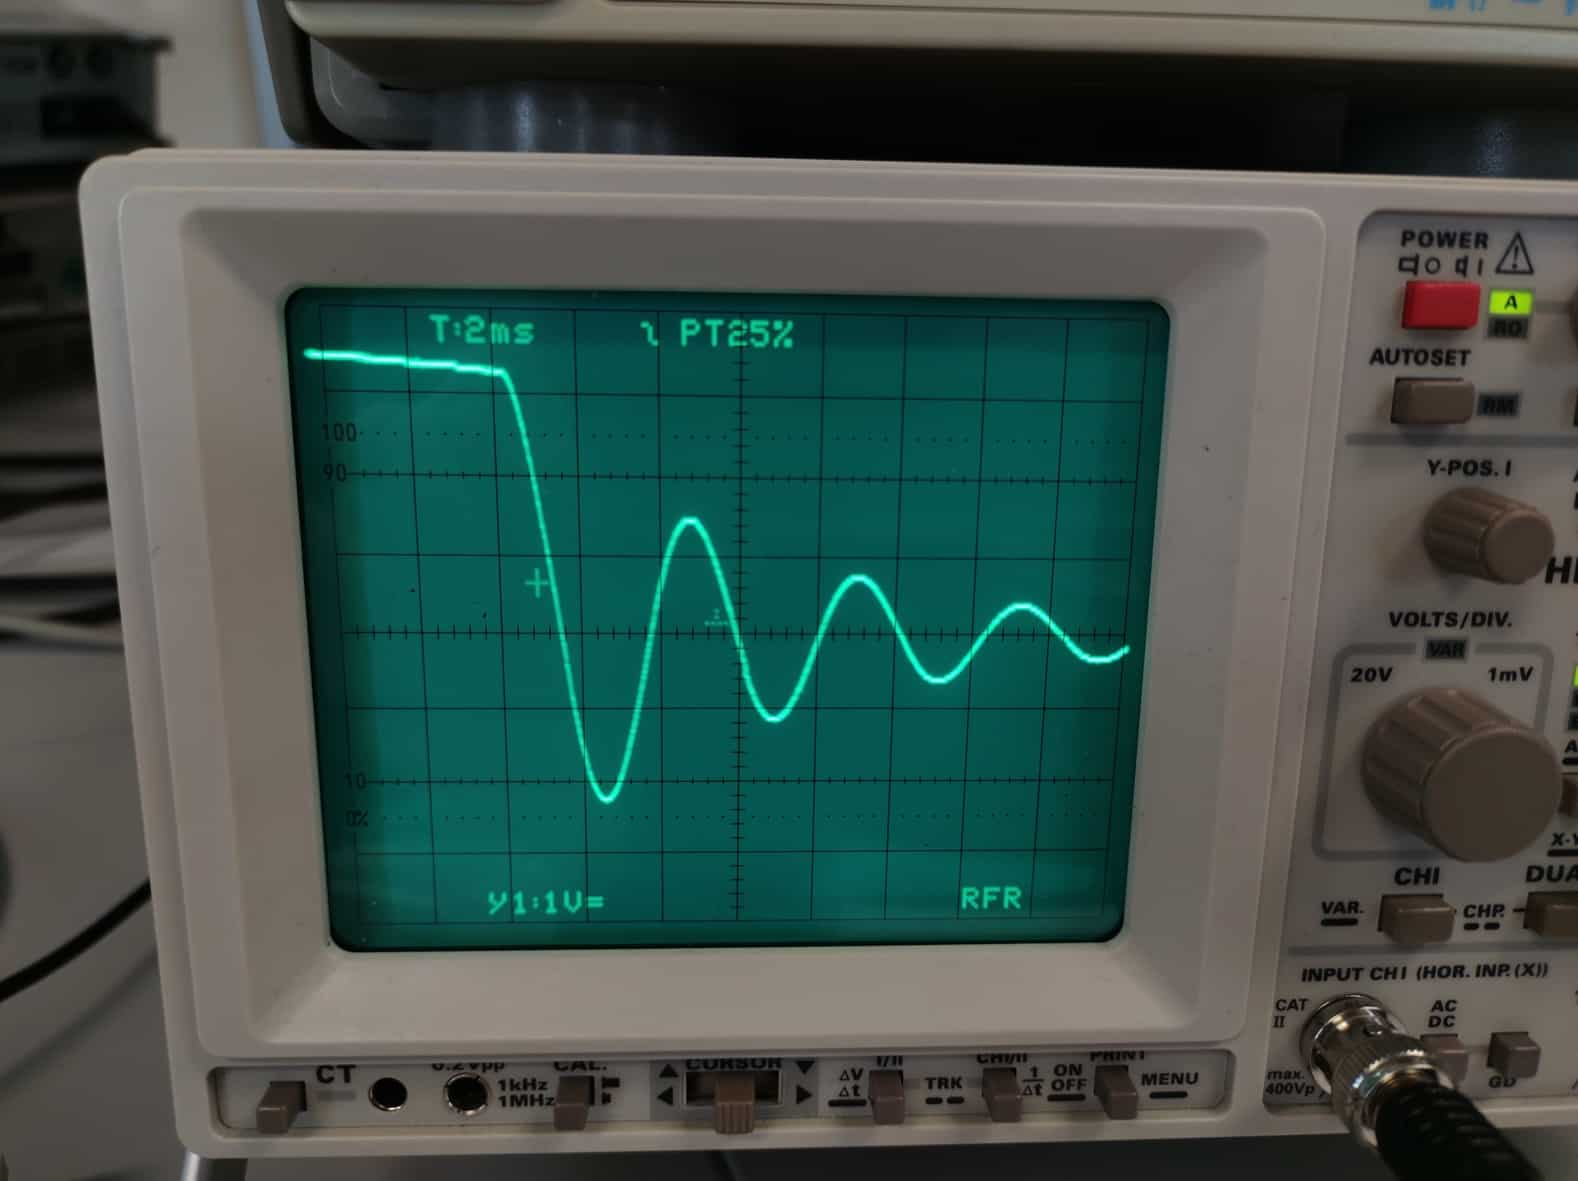
\includegraphics[width=8cm]{Bild_Osziloskop-Schwingung}
\centering
\end{figure}

\textbf{Aus dem Diagramm lässt sich ablesen:}
\begin{align*}
T_{D,\textit{exp.}} = (4,4\mp0,1)ms \\
A_{0,\textit{exp.}} = (3,2\mp0,1)V \\
A_{1,\textit{exp.}} = (1,5\mp0,1)V
\end{align*}

\textbf{Kreisfrequenz der gedämpften Schwingung:}
\begin{align}
\omega_{D,\textit{exp.}} = \frac{2\pi}{T_{D,\textit{exp.}}} = 1427,997
\end{align}

Fehlerrechnung:
\begin{align*}
\vert \frac{\partial}{\partial T_{D,\textit{exp.}}}\omega_{D,\textit{exp.}}\vert = \frac{2\pi}{T_{D,\textit{exp.}}^2}
\end{align*}
\begin{align*}
U_{\omega_{D,\textit{exp.}}} = \vert \frac{\partial}{\partial T_{D,\textit{exp.}}}\omega_{D,\textit{exp.}}\vert \cdot U_{T_{D,\textit{exp.}}} = 32,45 \approx 33 \frac{1}{s} 
\end{align*}

\begin{align*}
\Rightarrow \omega_{D,\textit{exp.}} = (1428 \mp 33) \frac{1}{s}
\end{align*}

\textbf{Berechnung des logarithmischen Dekrements:}
\begin{align}
\Lambda_{\textit{exp.}} = ln(\frac{A_{0,\textit{exp.}}}{A_{1,\textit{exp.}}}) = 0,7576
\end{align}

Fehlerrechnung:
\begin{align*}
\vert \frac{\partial}{\partial A_{0,\textit{exp.}}}\Lambda_{\textit{exp.}}\vert = \frac{1}{A_{0,\textit{exp.}}} \\
\vert \frac{\partial}{\partial A_{1,\textit{exp.}}}\Lambda_{\textit{exp.}}\vert = \frac{1}{A_{1,\textit{exp.}}}
\end{align*}
\begin{align*}
U_{\Lambda_{\textit{exp.}}} = \vert \frac{\partial}{\partial A_{0,\textit{exp.}}}\Lambda_{\textit{exp.}}\vert \cdot U_{A_{0,\textit{exp.}}} + \vert \frac{\partial}{\partial A_{1,\textit{exp.}}}\Lambda_{\textit{exp.}}\vert \cdot U_{A_{1,\textit{exp.}}} = 0,07569 \approx 0,076 
\end{align*}

\begin{align*}
\Rightarrow \Lambda_{\textit{exp.}} = (0,758 \mp 0,076)
\end{align*}

\textbf{Berechnung des Abklingkoeffizienten:}
\begin{align}
\delta_{\textit{exp.}} = \frac{\Lambda_{\textit{exp.}}}{T_{D,\textit{exp.}}} = 172,1818
\end{align}

Fehlerrechnung:
\begin{align*}
\vert \frac{\partial}{\partial \Lambda_{\textit{exp.}}}\delta_{\textit{exp.}}\vert = \frac{1}{T_{D,\textit{exp.}}} \\
\vert \frac{\partial}{\partial T_{D,\textit{exp.}}}\delta_{\textit{exp.}}\vert = \frac{\Lambda_{\textit{exp.}}}{T_{D,\textit{exp.}}^2}
\end{align*}

\begin{align*}
U_{\delta_{\textit{exp.}}} = \vert \frac{\partial}{\partial \Lambda_{\textit{exp.}}}\delta_{\textit{exp.}}\vert \cdot U_{\Lambda_{\textit{exp.}}} + \vert \frac{\partial}{\partial T_{D,\textit{exp.}}}\delta_{\textit{exp.}}\vert \cdot U_{T_{D,\textit{exp.}}} = 21,1859 \approx 22
\end{align*}

\begin{align*}
\Rightarrow \delta_{\textit{exp.}} = (172 \mp 22) \frac{1}{s}
\end{align*}

\subsubsection{Aperiodischer Grenzfall}

\begin{figure}[H]
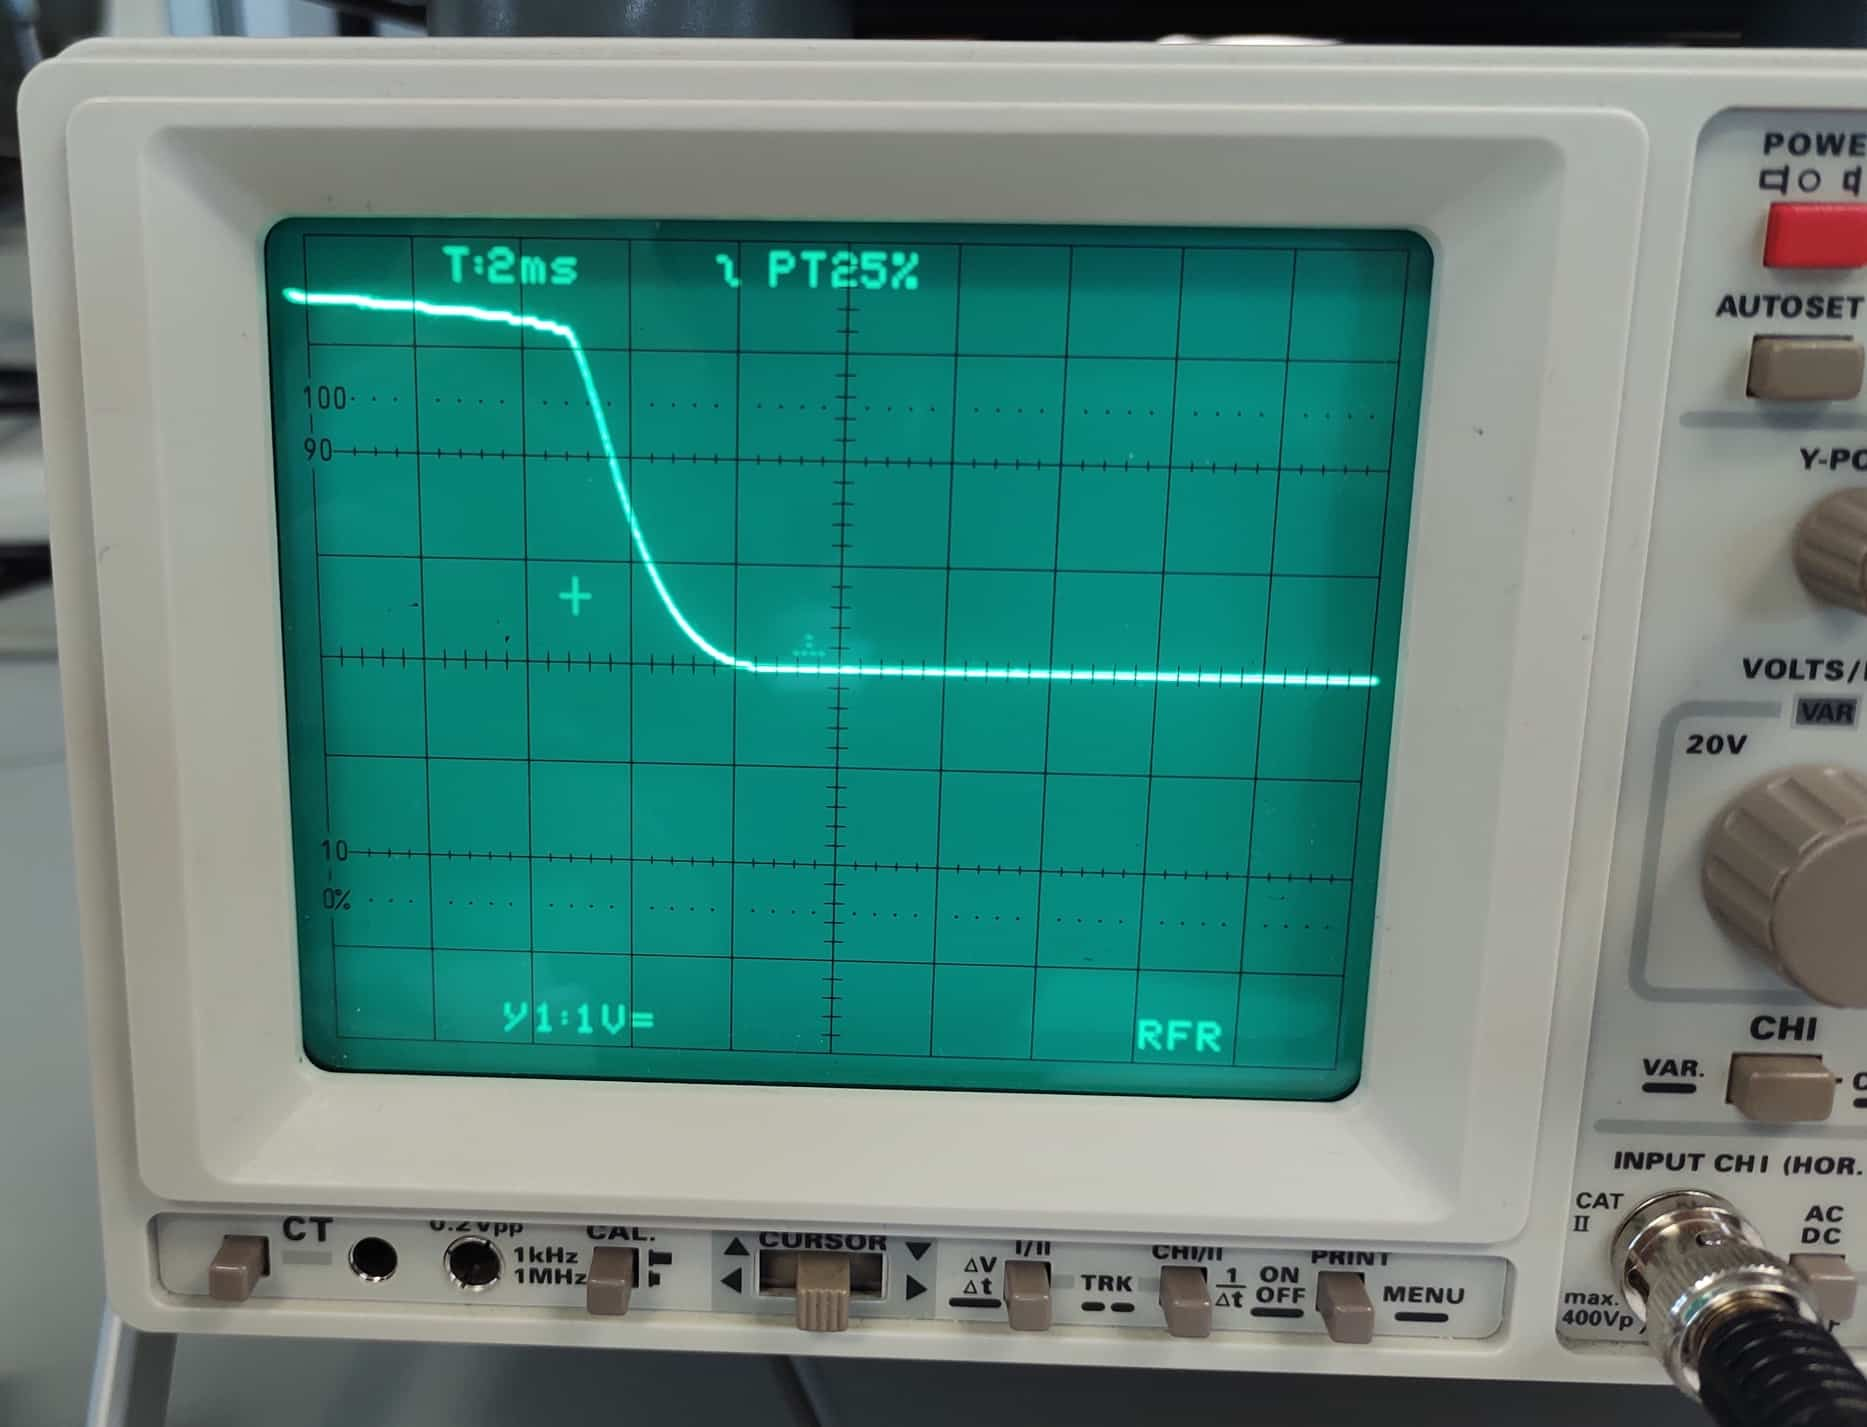
\includegraphics[width=8cm]{Bild_Osziloskop-Grenzfall}
\centering
\end{figure}

\textbf{Aus dem Diagramm lässt sich ablesen:}
\begin{align*}
R_{\textit{ext,exp.}} = (10,084\mp1,5)k\Omega
\end{align*}
Dabei wird als Messungenauigkeit $1,5k\Omega$ angenommen. Die Ungenauigkeit entsteht vor allem dadurch, dass sich der Widerstand in diesem Bereich verändern lässt, ohne, dass an dem Oszilloskop eine wesentlich Änderung erkennbar ist.

\textbf{Berechnung Gesamtwiderstand:}
\begin{align}
R_{\textit{ges,exp.}} = R_{\textit{ext,exp.}} + R_{\textit{int,exp.}} = 11,434k\Omega 
\end{align}

Fehlerrechnung:
\begin{align*}
U_{R_{\textit{ges,exp.}}} = U_{R_{\textit{ext,exp.}}} + U_{R_{\textit{int,exp.}}} = 1,551k\Omega \approx 1,6k\Omega
\end{align*}

\begin{align*}
\Rightarrow R_{\textit{ges,exp.}} = (11,4 \mp 1,6) k\Omega
\end{align*}

\end{document}
%%% Local Variables:
%%% mode: latex
%%% TeX-master: t
%%% End: